\documentclass[a4paper,12pt]{ctexart}

\usepackage[left=2.3cm,right=2.3cm,top=2.7cm,bottom=2.7cm]{geometry}
\usepackage{graphicx}
\usepackage{xcolor}
\usepackage{float}
\usepackage{booktabs}
\usepackage{array}
\usepackage{longtable}
\usepackage{tabularx}
\usepackage{amsmath,amssymb,bm}
\usepackage{fancyhdr}
\usepackage{lastpage}
\usepackage{hyperref}
\usepackage{pgfplots}
\usepackage{listings}
\usepackage{algorithm}
\usepackage{algorithmicx}
\usepackage{algpseudocode}

\pgfplotsset{compat=1.18}
\graphicspath{{images/}}

\hypersetup{
    colorlinks=true,
    linkcolor=black,
    urlcolor=blue,
    citecolor=black
}

\lstset{
    language=C++,
    breaklines=true,
    basicstyle=\small\ttfamily,
    keywordstyle=\color{blue!70}\bfseries,
    commentstyle=\color{green!40!black},
    stringstyle=\color{red!60!black},
    numbers=left,
    numberstyle=\tiny\color{blue!50},
    frame=single,
    columns=flexible,
    showstringspaces=false
}

\floatname{algorithm}{Algorithm}
\renewcommand{\algorithmicrequire}{\textbf{Input:}}
\renewcommand{\algorithmicensure}{\textbf{Output:}}

\makeatletter
\newenvironment{breakablealgorithm}
  {
   \begin{center}
     \refstepcounter{algorithm}
     \hrule height .8pt depth 0pt \kern 2pt
     \renewcommand{\caption}[2][\relax]{
       {\raggedright\textbf{\ALG@name~\thealgorithm} ##2\par}
       \ifx\relax##1\relax
         \addcontentsline{loa}{algorithm}{\protect\numberline{\thealgorithm}##2}
       \else
         \addcontentsline{loa}{algorithm}{\protect\numberline{\thealgorithm}##1}
       \fi
       \kern2pt\hrule\kern2pt
     }
  }
  {
     \kern2pt\hrule\relax
   \end{center}
  }
\makeatother

\newcommand{\HRule}{\rule{\linewidth}{0.5mm}}
\newcommand{\HRulegrossa}{\rule{\linewidth}{1.2mm}}

\pagestyle{fancy}
\fancyhf{}
\lhead{\kaishu \leftmark}
\rhead{\kaishu 并行程序设计实验报告}
\cfoot{\thepage\ / \pageref{LastPage}}
\renewcommand{\headrulewidth}{0.1pt}
\renewcommand{\footrulewidth}{0pt}

\renewcommand{\contentsname}{目录}
\renewcommand{\refname}{参考文献}
\renewcommand{\figurename}{图}
\renewcommand{\tablename}{表}
\renewcommand{\today}{\number\year 年 \number\month 月 \number\day 日}
\setcounter{tocdepth}{2}
\begin{document}

\begin{titlepage}
    \begin{center}
        
\includegraphics[width=0.8\textwidth]{NKU.png}\\[1cm]

        \vspace{20mm}

        {\huge\bfseries\kaishu 计算机学院\par}
        \vspace{0.5cm}
        {\huge\bfseries\kaishu 并行程序设计实验报告\par}
        \vspace{2.3cm}
        {\Huge\bfseries\kaishu n个数求和的链式、指令级并行与树形归约算法实验\par}

        \vspace{\fill}

        {\LARGE\kaishu 姓名：马禹翔\par}
        \vspace{0.5cm}
        {\LARGE\kaishu 学号：2410933\par}
        \vspace{0.5cm}
        {\LARGE\kaishu 专业：计算机科学与技术\par}

        \vfill
        {\Large \today\par}
    \end{center}
\end{titlepage}

\tableofcontents
\thispagestyle{plain}
\clearpage

\section*{代码仓库说明}

本实验完整源码已上传至 GitHub，访问地址如下：

\begin{center}
\url{https://github.com/s1nk141/nku26/blob/create/lab1_2.zip}
\end{center}

\section{实验目的}

本实验围绕“计算 $n$ 个数之和”这一基础问题，比较不同算法结构在现代处理器上的性能表现，具体目标如下：

\begin{enumerate}
  \item 理解平凡链式累加算法的计算过程及其数据依赖特性；
  \item 掌握两路链式累加算法的基本思想，理解其如何通过减少依赖链长度提升指令级并行潜力；
  \item 理解树形归约算法的计算结构，分析其适合并行化实现的原因；
  \item 学会使用 \texttt{chrono} 进行高精度计时，并通过重复多次测量减少误差；
  \item 通过实验数据比较不同算法在串行与并行实现下的实际性能差异，分析理论并行性与实际运行效果之间的关系。
\end{enumerate}

\section{实验原理}

\subsection{问题描述}

设数组为 $p$，长度为 $N$，实验要求计算：

\begin{equation}
S=\sum_{i=0}^{N-1}p[i]
\end{equation}

其中本实验中令：

\begin{equation}
p[i]=i
\end{equation}

并取：

\begin{equation}
N=2^n
\end{equation}

这样做一方面便于验证结果正确性，另一方面也方便树形归约算法按层次不断折半。

\subsection{平凡链式累加算法}

最直接的求和方法是逐个元素累加：

\begin{equation}
sum=sum+p[i]
\end{equation}

该方法结构简单，只需一次线性扫描即可完成全部求和，但它存在严格的循环携带依赖。因为下一次加法必须依赖前一次更新后的 $sum$，所以形成了一条长度为 $N$ 的依赖链。在并行视角下，其关键路径长度为 $O(N)$。

\subsection{两路链式累加与指令级并行}

为了降低依赖链长度，可以引入两个独立累加器：

\begin{equation}
sum_1=sum_1+p[i],\quad sum_2=sum_2+p[i+1]
\end{equation}

最后再执行一次：

\begin{equation}
sum=sum_1+sum_2
\end{equation}

这样原本单一的依赖链被拆分为两条较短的独立链。由于 \texttt{sum1} 与 \texttt{sum2} 之间互不依赖，处理器有机会同时调度这两条加法指令，从而更好地利用超标量处理器中的多个执行单元。这种优化属于典型的指令级并行优化。

\subsection{树形归约算法}

树形归约的基本思想是先将相邻两个元素相加，再对得到的中间结果继续两两相加，如此反复，直到只剩下一个结果。其形式可表示为：

\begin{equation}
p[i]=p[2i]+p[2i+1]
\end{equation}

每进行一轮，有效数据规模缩小为原来的一半，因此总共只需要：

\begin{equation}
\log_2 N
\end{equation}

轮归约。与链式算法相比，树形归约将关键路径长度从 $O(N)$ 缩短为 $O(\log N)$，理论并行性更强。

\subsection{并行树形归约}

在树形归约的每一轮中，所有形如

\begin{equation}
p[i]=p[2i]+p[2i+1]
\end{equation}

的操作彼此独立，因此可以利用 OpenMP 对每一层内部的循环进行并行化。这样，外层按层次逐轮推进，内层由多个线程同时完成本层的配对求和。

不过，树形归约虽然更适合并行，但这并不意味着它在实际 CPU 上一定快于普通线性求和。其性能还会受到线程调度、同步开销、数组写回开销以及问题规模等因素影响。:contentReference[oaicite:2]{index=2}

\section{实验平台与实验方案}

\subsection{实验平台}

本实验在 Ubuntu 环境下完成，采用 C++ 编写程序，并使用 OpenMP 实现并行树形归约。实验平台配置如下：

操作系统：Ubuntu

编译器：g++

编译选项：\texttt{-O2 -fopenmp -std=c++11}

并行库：OpenMP

\subsection{测试数据设计}

为保证结果可复现，本实验采用固定方式初始化数组：

\begin{equation}
p[i]=i
\end{equation}

此时理论正确结果为：

\begin{equation}
S=0+1+2+\cdots+(N-1)=\frac{N(N-1)}{2}
\end{equation}

该构造方式简单明确，便于人工核对结果。:contentReference[oaicite:3]{index=3}

\subsection{测试规模设计}

根据实验要求与内存开销情况，本实验选取如下问题规模进行测试：

\begin{enumerate}
  \item $n=15$，即 $N=2^{15}=32768$
  \item $n=20$，即 $N=2^{20}=1048576$
  \item $n=24$，即 $N=2^{24}=16777216$
\end{enumerate}

这样既能够覆盖中小规模与较大规模输入，也能观察随着规模增大，各算法性能变化的趋势。:contentReference[oaicite:4]{index=4}

\subsection{计时方法}

实验采用 \texttt{chrono::high\_resolution\_clock} 进行高精度计时，计时单位为纳秒（ns）。为减少单次测量波动带来的误差，每个算法在同一输入规模下重复执行 10 次，并取平均值作为最终运行时间。

此外，程序使用 \texttt{volatile long long sink} 接收函数返回值，以避免编译器在 \texttt{-O2} 优化下将无副作用的计算直接消除，从而保证计时结果具有可信度。:contentReference[oaicite:5]{index=5}

\section{算法设计与代码实现}

\subsection{算法思路说明}

本实验共实现四种求和算法：

\begin{enumerate}
  \item \textbf{平凡算法 ordinary\_alg}：使用单个累加器按顺序逐个累加；
  \item \textbf{两路链式累加算法 ilp\_alg}：使用两个独立累加器，体现指令级并行思想；
  \item \textbf{树形归约算法 optimized\_alg}：采用原地两两相加、逐层折半的方式求和；
  \item \textbf{并行树形归约算法 parallel\_alg}：在树形归约每一层内部使用 OpenMP 并行化。
\end{enumerate}

这四种算法分别对应不同的结构优化思路，因此能够较全面地体现“平凡算法—ILP 优化—树形归约—并行实现”的演进过程。:contentReference[oaicite:6]{index=6}

\subsection{核心代码}

下面给出本实验的完整代码。

\begin{lstlisting}[title=完整实验代码]
#include<iostream>
#include<chrono>
#include<vector>
#include<omp.h>

using namespace std;
using namespace std::chrono;

void init_data(vector<long long>& p) {
    for (int i = 0; i < p.size(); i++) {
        p[i] = i;
    }
}

long long ordinary_alg(vector<long long>& p) {
    long long sum = 0;
    for (int i = 0; i < p.size(); i++) {
        sum += p[i];
    }
    return sum;
}

long long ilp_alg(vector<long long>& p) {
    long long sum1 = 0;
    long long sum2 = 0;
    int i = 0;
    for (; i + 1 < p.size(); i += 2) {
        sum1 += p[i];
        sum2 += p[i + 1];
    }
    if (i < p.size()) {
        sum1 += p[i];
    }
    return sum1 + sum2;
}

long long optimized_alg(vector<long long>& p) {
    int m = p.size();
    for (int n = m; n > 1; n = n / 2) {
        for (int i = 0; i < n / 2; i++) {
            p[i] = p[2 * i] + p[2 * i + 1];
        }
    }
    return p[0];
}

long long parallel_alg(vector<long long>& p) {
    int m = p.size();
    for (int n = m; n > 1; n = n / 2) {
#pragma omp parallel for
        for (int i = 0; i < n / 2; i++) {
            p[i] = p[2 * i] + p[2 * i + 1];
        }
    }
    return p[0];
}

int main() {
    int n;
    cout << "please cin the amount of n" << endl;
    cin >> n;

    int s = 1 << n;
    vector<long long> p(s, -1);
    init_data(p);

    volatile long long sink = 0;

    long long total1 = 0;
    long long total2 = 0;
    long long total3 = 0;
    long long total4 = 0;

    int r = 10;

    for (int i = 0; i < r; i++) {
        auto start1 = high_resolution_clock::now();
        sink = ordinary_alg(p);
        auto end1 = high_resolution_clock::now();
        total1 += duration_cast<nanoseconds>(end1 - start1).count();

        auto start2 = high_resolution_clock::now();
        sink = ilp_alg(p);
        auto end2 = high_resolution_clock::now();
        total2 += duration_cast<nanoseconds>(end2 - start2).count();

        vector<long long> temp = p;
        auto start3 = high_resolution_clock::now();
        sink = optimized_alg(temp);
        auto end3 = high_resolution_clock::now();
        total3 += duration_cast<nanoseconds>(end3 - start3).count();

        vector<long long> temp2 = p;
        auto start4 = high_resolution_clock::now();
        sink = parallel_alg(temp2);
        auto end4 = high_resolution_clock::now();
        total4 += duration_cast<nanoseconds>(end4 - start4).count();
    }

    double average_time1 = 1.0 * total1 / r;
    double average_time2 = 1.0 * total2 / r;
    double average_time3 = 1.0 * total3 / r;
    double average_time4 = 1.0 * total4 / r;

    cout << "the answer of ordinary_alg is: " << ordinary_alg(p) << endl;
    cout << "the time cost of ordinary_alg is: " << average_time1 << endl;

    cout << "the answer of ilp_alg is: " << ilp_alg(p) << endl;
    cout << "the time cost of ilp_alg is: " << average_time2 << endl;

    vector<long long> temp = p;
    cout << "the answer of optimized_alg is: " << optimized_alg(temp) << endl;
    cout << "the time cost of optimized_alg is: " << average_time3 << endl;

    vector<long long> temp2 = p;
    cout << "the answer of parallel_alg is: " << parallel_alg(temp2) << endl;
    cout << "the time cost of parallel_alg is: " << average_time4 << endl;

    cout << "speed up of ilp_alg: " << average_time1 / average_time2 << endl;
    cout << "speed up of optimized_alg: " << average_time1 / average_time3 << endl;
    cout << "speed up of parallel_alg: " << average_time1 / average_time4 << endl;

    return 0;
}
\end{lstlisting}

\subsection{代码结构与关键实现解析}

\subsubsection{数据初始化}

\begin{lstlisting}
void init_data(vector<long long>& p) {
    for (int i = 0; i < p.size(); i++) {
        p[i] = i;
    }
}
\end{lstlisting}

该函数用于生成测试数据，将数组初始化为 $p[i]=i$。由于数据分布规则明确，便于验证结果正确性，并能避免随机数据引入的额外不确定性。

\subsubsection{平凡算法}

\begin{lstlisting}
long long ordinary_alg(vector<long long>& p) {
    long long sum = 0;
    for (int i = 0; i < p.size(); i++) {
        sum += p[i];
    }
    return sum;
}
\end{lstlisting}

平凡算法使用单个累加器依次累加所有元素。其优点是代码简单、访存连续、局部变量可保留在寄存器中；其缺点是存在严格的循环依赖，不利于指令级并行。

\subsubsection{两路链式累加算法}

\begin{lstlisting}
long long ilp_alg(vector<long long>& p) {
    long long sum1 = 0;
    long long sum2 = 0;
    int i = 0;
    for (; i + 1 < p.size(); i += 2) {
        sum1 += p[i];
        sum2 += p[i + 1];
    }
    if (i < p.size()) {
        sum1 += p[i];
    }
    return sum1 + sum2;
}
\end{lstlisting}

该算法引入两个独立累加器 \texttt{sum1} 和 \texttt{sum2}，从而将原本的一条长依赖链拆成两条较短的依赖链。这种结构更适合超标量处理器利用多个执行单元进行指令调度，体现了指令级并行思想。

\subsubsection{树形归约算法}

\begin{lstlisting}
long long optimized_alg(vector<long long>& p) {
    int m = p.size();
    for (int n = m; n > 1; n = n / 2) {
        for (int i = 0; i < n / 2; i++) {
            p[i] = p[2 * i] + p[2 * i + 1];
        }
    }
    return p[0];
}
\end{lstlisting}

树形归约算法按层次将相邻两个元素合并，并将结果原地写回数组前半部分。该算法理论并行性较强，但其串行实现需要多轮循环，并且每轮都涉及数组写回，因此常数开销较大。

\subsubsection{并行树形归约算法}

\begin{lstlisting}
long long parallel_alg(vector<long long>& p) {
    int m = p.size();
    for (int n = m; n > 1; n = n / 2) {
#pragma omp parallel for
        for (int i = 0; i < n / 2; i++) {
            p[i] = p[2 * i] + p[2 * i + 1];
        }
    }
    return p[0];
}
\end{lstlisting}

并行树形归约算法利用 OpenMP 对每一轮内部的归约操作进行并行调度。由于同一层的各个配对求和任务互不依赖，因此适合并行执行。但线程创建、调度与同步也会带来额外开销，尤其在问题规模较小时影响更明显。

\subsubsection{计时逻辑}

\begin{lstlisting}
for (int i = 0; i < r; i++) {
    auto start1 = high_resolution_clock::now();
    sink = ordinary_alg(p);
    auto end1 = high_resolution_clock::now();
    total1 += duration_cast<nanoseconds>(end1 - start1).count();

    auto start2 = high_resolution_clock::now();
    sink = ilp_alg(p);
    auto end2 = high_resolution_clock::now();
    total2 += duration_cast<nanoseconds>(end2 - start2).count();

    vector<long long> temp = p;
    auto start3 = high_resolution_clock::now();
    sink = optimized_alg(temp);
    auto end3 = high_resolution_clock::now();
    total3 += duration_cast<nanoseconds>(end3 - start3).count();

    vector<long long> temp2 = p;
    auto start4 = high_resolution_clock::now();
    sink = parallel_alg(temp2);
    auto end4 = high_resolution_clock::now();
    total4 += duration_cast<nanoseconds>(end4 - start4).count();
}
\end{lstlisting}

程序对每种算法重复执行 10 次并统计总耗时，最终求平均值。由于 \texttt{optimized\_alg} 和 \texttt{parallel\_alg} 会修改数组，因此在调用前先复制一份原数组，以保证每次测试的输入一致。:contentReference[oaicite:7]{index=7}

\subsection{伪代码描述}

\begin{breakablealgorithm}
\caption{n个数求和的四种实现方式}
\begin{algorithmic}[1]
\Require 数组 $p$
\Ensure 数组元素总和
\Function{OrdinaryAlg}{$p$}
    \State $sum\gets 0$
    \For{$i=0$ to $N-1$}
        \State $sum\gets sum+p[i]$
    \EndFor
    \State \Return $sum$
\EndFunction

\Function{ILPAlg}{$p$}
    \State $sum_1\gets 0,\ sum_2\gets 0$
    \For{$i=0$ to $N-2$ step 2}
        \State $sum_1\gets sum_1+p[i]$
        \State $sum_2\gets sum_2+p[i+1]$
    \EndFor
    \If{$N$ 为奇数}
        \State $sum_1\gets sum_1+p[N-1]$
    \EndIf
    \State \Return $sum_1+sum_2$
\EndFunction

\Function{OptimizedAlg}{$p$}
    \State $n\gets N$
    \While{$n>1$}
        \For{$i=0$ to $n/2-1$}
            \State $p[i]\gets p[2i]+p[2i+1]$
        \EndFor
        \State $n\gets n/2$
    \EndWhile
    \State \Return $p[0]$
\EndFunction

\Function{ParallelAlg}{$p$}
    \State $n\gets N$
    \While{$n>1$}
        \State 并行执行以下循环
        \For{$i=0$ to $n/2-1$}
            \State $p[i]\gets p[2i]+p[2i+1]$
        \EndFor
        \State $n\gets n/2$
    \EndWhile
    \State \Return $p[0]$
\EndFunction
\end{algorithmic}
\end{breakablealgorithm}

\section{实验结果}

在当前实验平台下，得到如下测试结果。每组数据均重复运行 10 次并取平均值。

\begin{table}[H]
\centering
\begin{tabular}{ccccc}
\toprule
$n$ & ordinary\_alg(ns) & ilp\_alg(ns) & optimized\_alg(ns) & parallel\_alg(ns) \\
\midrule
5  & 111.2 & 152.3 & 169.4 & $1.41967\times 10^{4}$ \\
10 & 936.7 & 693.4 & 1512.9 & $2.41351\times 10^{4}$ \\
15 & $1.97160\times 10^{4}$ & $1.69047\times 10^{4}$ & $4.03892\times 10^{4}$ & $6.85470\times 10^{4}$ \\
20 & $1.43018\times 10^{6}$ & $9.81512\times 10^{5}$ & $3.62507\times 10^{6}$ & $3.19072\times 10^{6}$ \\
25 & $8.49219\times 10^{7}$ & $2.77975\times 10^{7}$ & $2.03020\times 10^{8}$ & $8.23004\times 10^{7}$ \\
\bottomrule
\end{tabular}
\caption{不同规模下各算法平均运行时间}
\label{table:result1}
\end{table}

根据程序输出可进一步得到加速比：

\begin{table}[H]
\centering
\begin{tabular}{cccc}
\toprule
$n$ & ilp\_alg加速比 & optimized\_alg加速比 & parallel\_alg加速比 \\
\midrule
5  & 1.177 & 1.059 & 0.012 \\
10 & 1.350 & 0.619 & 0.038 \\
15 & 1.166 & 0.488 & 0.287 \\
20 & 1.457 & 0.394 & 0.448 \\
25 & 3.055 & 0.418 & 1.031 \\
\bottomrule
\end{tabular}
\caption{相对于ordinary\_alg的加速比}
\label{table:result2}
\end{table}

\begin{figure}[H]
\centering
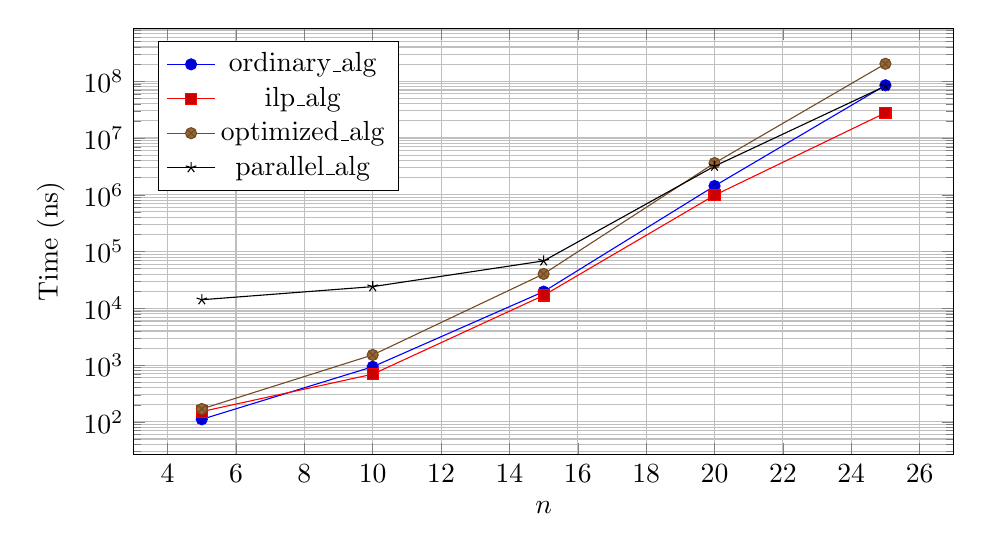
\begin{tikzpicture}
\begin{axis}[
    xlabel={$n$},
    ylabel={Time (ns)},
    ymode=log,
    log basis y={10},
    legend pos=north west,
    grid=both,
    width=12cm,
    height=7cm
]

\addplot coordinates {
(5,111.2)
(10,936.7)
(15,1.97160e4)
(20,1.43018e6)
(25,8.49219e7)
};
\addlegendentry{ordinary\_alg}

\addplot coordinates {
(5,152.3)
(10,693.4)
(15,1.69047e4)
(20,9.81512e5)
(25,2.77975e7)
};
\addlegendentry{ilp\_alg}

\addplot coordinates {
(5,169.4)
(10,1512.9)
(15,4.03892e4)
(20,3.62507e6)
(25,2.03020e8)
};
\addlegendentry{optimized\_alg}

\addplot coordinates {
(5,1.41967e4)
(10,2.41351e4)
(15,6.85470e4)
(20,3.19072e6)
(25,8.23004e7)
};
\addlegendentry{parallel\_alg}

\end{axis}
\end{tikzpicture}
\caption{不同算法运行时间对比}
\end{figure}

\begin{figure}[H]
\centering
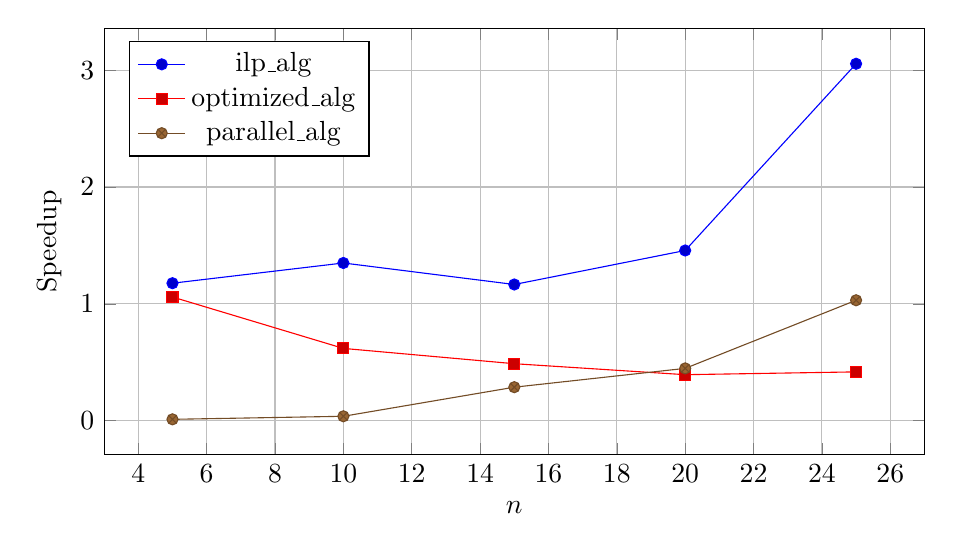
\begin{tikzpicture}
\begin{axis}[
    xlabel={$n$},
    ylabel={Speedup},
    grid=both,
    width=12cm,
    height=7cm,
    legend pos=north west
]

\addplot coordinates {
(5,1.177)
(10,1.350)
(15,1.166)
(20,1.457)
(25,3.055)
};
\addlegendentry{ilp\_alg}

\addplot coordinates {
(5,1.059)
(10,0.619)
(15,0.488)
(20,0.394)
(25,0.418)
};
\addlegendentry{optimized\_alg}

\addplot coordinates {
(5,0.012)
(10,0.038)
(15,0.287)
(20,0.448)
(25,1.031)
};
\addlegendentry{parallel\_alg}

\end{axis}
\end{tikzpicture}
\caption{不同优化算法加速比变化}
\end{figure}

从实验结果可以看出，不同算法在不同问题规模下表现差异明显。两路链式累加算法在各组测试中均优于平凡算法，且随着规模增大优势更加明显；树形归约串行实现始终慢于平凡算法；OpenMP 并行树形归约在小规模下开销很大，在较大规模下性能逐渐改善，并在 $n=25$ 时略微超过 ordinary\_alg。:contentReference[oaicite:8]{index=8}

\section{实验过程中遇到的问题与解决方法}

在实验过程中，先后遇到了若干典型问题，这些问题本身也帮助加深了对算法与体系结构关系的理解。

\subsection{树形归约结果出错}

最初实现树形归约时，数组类型使用的是 \texttt{int}。当问题规模增大时，中间归约结果已经远远超过 \texttt{int} 的取值范围，导致程序输出负值或错误结果。后来将数组类型改为 \texttt{long long}，问题得到解决。这说明在并行或归约问题中，不仅最终结果范围要考虑，中间结果范围同样不能忽视。:contentReference[oaicite:9]{index=9}

\subsection{对“优化”概念的理解偏差}

实验初期容易误认为只要算法在理论上更适合并行，其串行实现也应当更快。但实际测试表明并非如此。树形归约优化的重点是“关键路径更短、并行潜力更大”，而 ordinary\_alg 优化的是“串行执行路径极简、常数开销极小”。这两种“优化”面向的是不同层面的性能目标，不能简单混为一谈。:contentReference[oaicite:10]{index=10}

\section{结论}

本实验围绕 n 个数求和问题，实现并比较了平凡链式累加、两路链式累加、树形归约以及 OpenMP 并行树形归约四种算法。结合理论分析与实验结果，可以得到以下结论：

\begin{enumerate}
  \item 平凡链式累加算法结构简单、访存连续，在小规模和中等规模下具有较好的基线性能；
  \item 两路链式累加算法通过引入两个独立累加器，降低了依赖链长度，较好地体现了指令级并行优化思想，并且在本实验所有测试规模下都优于平凡算法，是本次实验中综合表现最好的优化方法；
  \item 树形归约算法虽然理论上将关键路径由 $O(N)$ 缩短为 $O(\log N)$，具有较强的并行潜力，但其串行实现由于多轮循环、索引计算和数组写回，实际开销较大，在本实验中始终慢于平凡算法；
  \item OpenMP 并行树形归约在小规模下受到线程调度与同步开销影响，性能明显不佳；随着问题规模增大，其性能逐渐提升，并在 $n=25$ 时略微超过平凡算法，说明树形归约的并行优势需要足够大的问题规模才能体现；
  \item 程序性能不仅取决于算法的渐进复杂度，还受到数据依赖、访存方式、编译器优化以及并行实现开销的共同影响。
\end{enumerate}
综上，本实验较系统地展示了从链式累加到指令级并行，再到树形归约和并行归约的算法演进过程。实验结果表明，在当前 CPU 平台上，两路链式累加这种面向单核执行的指令级并行优化最有效；而树形归约的优势更多体现在大规模并行执行场景中，而不是简单的串行实现中。这说明在实际程序优化中，需要根据硬件平台和问题规模选择合适的优化策略，而不能仅依据理论并行性判断算法优劣。

\end{document}